\documentclass[12pt]{article}
\usepackage[T1]{fontenc}
\usepackage[T1]{polski}
\usepackage[utf8]{inputenc}
\newcommand{\BibTeX}{{\sc Bib}\TeX} 
\usepackage{graphicx}
\usepackage{amsfonts}
\usepackage{amsmath}
\usepackage{latexsym}
\usepackage{float}

\setlength{\textheight}{21cm}

\title{{\bf Zadanie nr 4 }\linebreak
Cyfrowe Przetwarzanie Sygnałów}
\author{Dawid Jakubik, 224307 \and Hubert Gawłowski, 224298}
\date{17.06.2021}

\begin{document}
\clearpage\maketitle
\thispagestyle{empty}
\newpage
\setcounter{page}{1}
\section{Cel zadania}

Celem zadania było zapoznanie się z operacjami transformacji sygnałów dyskretnych przy użyciu wybranych metod oraz zaimplementowanie tychże metod w celu wygenerowania odpowiednich transformat.

\section{Wstęp teoretyczny}
Podczas pracy nad zadaniem korzystaliśmy z teorii zawartej w instrukcji na platformie Wikamp \cite{instrukcja}. Znajdują się w niej wszystkie potrzebne wzory dotyczące interesujących nas transformacji.
Oczywiście, zgodnie z instrukcją zapewniliśmy dwa tryby wyświetlania wykresu:
\begin{itemize}
    \item (W1) - górny wykres prezentuje część rzeczywistą amplitudy w funkcji częstotliwości, a wykres dolny część urojoną.
    \item (W2) - górny wykres prezentuje moduł liczby zespolonej, a dolny argument liczby w funkcji częstotliwości.
\end{itemize}
W ramach zadania zaimplementowaliśmy wymienione w instrukcji transformacje sygnałów. Z racji numerów indeksów przydzielony nam został Zestaw 2, a więc wariant transformacji falkowej (DB4)


\section{Eksperymenty i wyniki}

%%%%%%%%%%%%%%%%%%%%%%%%%%%%%%%%%%%%%%%%%%%%%%%%%%%%%%%%%%%%%%%%%%%%%%%%%%%%%%%%%%%%%%%%%%%%%%%%%%%%%%%%%%%%%%%%%
% PODROZDZIA£ PT. EKSPERYMENT NR 1 
%%%%%%%%%%%%%%%%%%%%%%%%%%%%%%%%%%%%%%%%%%%%%%%%%%%%%%%%%%%%%%%%%%%%%%%%%%%%%%%%%%%%%%%%%%%%%%%%%%%%%%%%%%%%%%%%%

\subsection{Wykresy wejściowe}

Na początek wygenerowaliśmy wykresy o następujących wzorach, na których będą przeprowadzane transformacje:
\begin{itemize}
    \item (S1):
    \begin{equation}
        S(t) = 2 \sin (\frac{2 \pi}{2}t + \frac{\pi}{2}) + 5 \sin (\frac{2 \pi}{0.5}t + \frac{\pi}{2})f_{pr} = 16
    \end{equation}
    \item (S2):
    \begin{equation}
        S(t) = 2 \sin (\frac{2 \pi}{2}t) + \sin (\frac{2 \pi}{1}t)+5 \sin (\frac{2\pi}{0.5}t) f_{pr} = 16
    \end{equation}
    \item (S3):
    \begin{equation}
        S(t) = 5 \sin (\frac{2 \pi}{2}t) + \sin (\frac{2 \pi}{0.25}t)f_{pr} = 16
    \end{equation}
\end{itemize}

% zeby wygenerować podałem dla sinusoidalnych wartosci:
% Pierwszy: A:2, ts: 1.39, czas trwania:4, T:2
% Drugi: A:5, ts:1.39, czas trwania:4, T:0.5
Wygenerowane wykresy przedstawiają się następująco:
\begin{figure}[H]
	\centering
	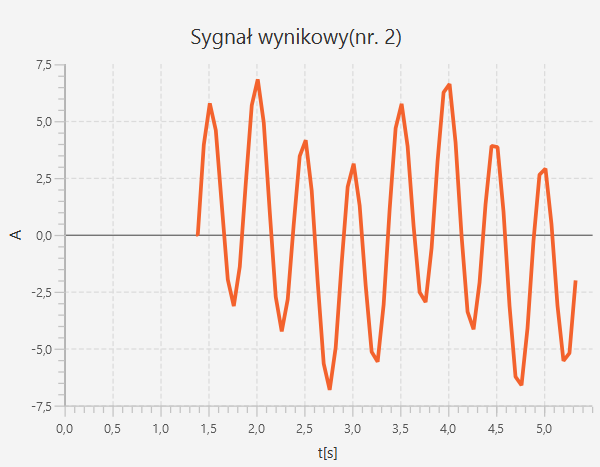
\includegraphics[width=\linewidth]{S1.png}
	\caption{Wykres sygnału S1}
	\label{S1_sygnal}
\end{figure}

% zeby wygenerować podałem dla sinusoidalnych wartosci:
% Pierwszy: A:2, ts: 0, czas trwania:4, T:2
% Drugi: A:1, ts:0, czas trwania:4, T:1
% i potem klkinałem "Dodaj do wygenrowanego; wtedy dodaje do shardkodowanego sygnału
\begin{figure}[H]
	\centering
	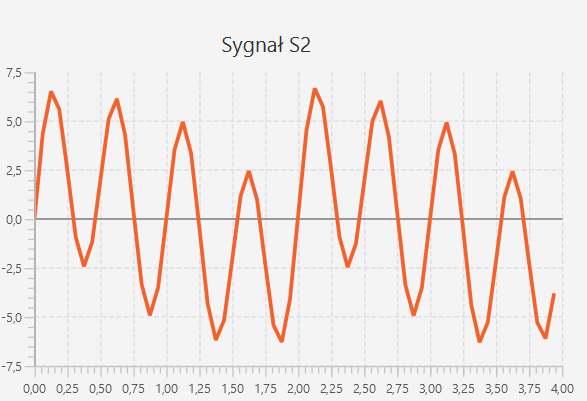
\includegraphics[width=\linewidth]{S2.png}
	\caption{Wykres sygnału S2}
	\label{S2_sygnal}
\end{figure}

% zeby wygenerować podałem dla sinusoidalnych wartosci:
% Pierwszy: A:5, ts: 0, czas trwania:4, T:2
% Drugi: A:1, ts:0, czas trwania:4, T:0.25

\begin{figure}[H]
	\centering
	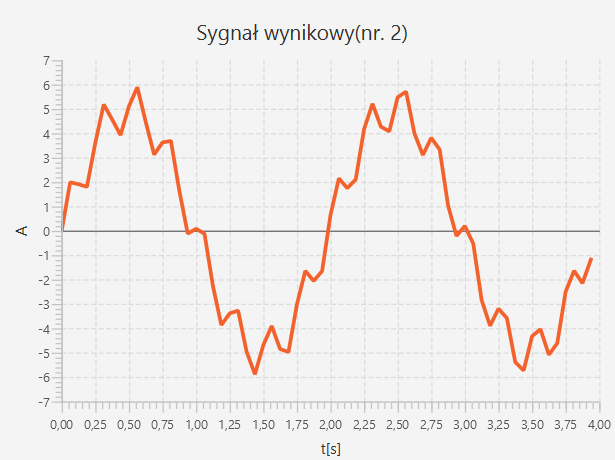
\includegraphics[width=\linewidth]{S3.png}
	\caption{Wykres sygnału S3}
	\label{S3_sygnal}
\end{figure}


\subsection {Dyskretna transformata Fouriera}
\begin{figure}[H]
	\centering
	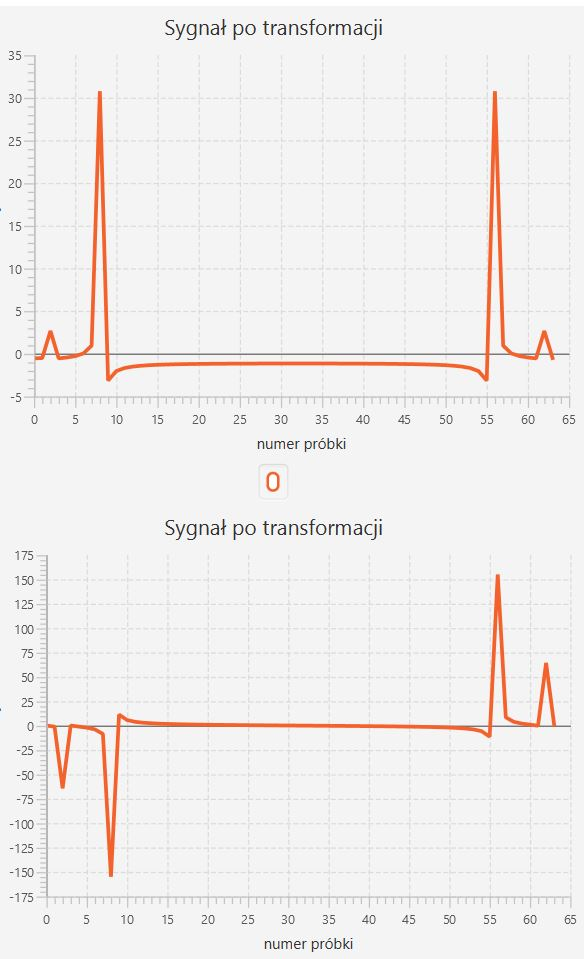
\includegraphics[width=.8\linewidth]{DFT-S1-W1}
	\caption{Wykresy w formie W1 DFT dla sygnału S1. Czas obliczania: 1118799}
	\label{S1_sygnal}
\end{figure}
\begin{figure}[H]
	\centering
	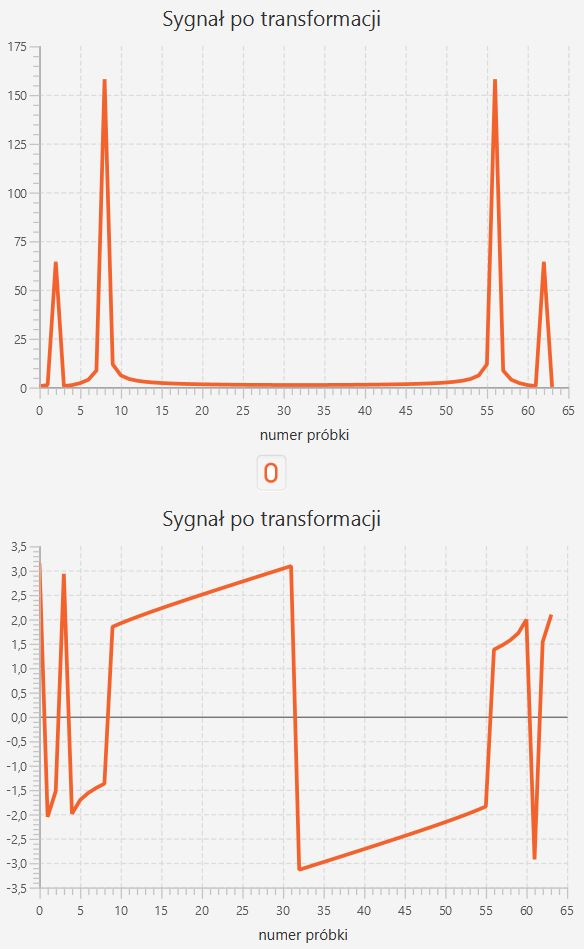
\includegraphics[width=.8\linewidth]{DFT-S1-W2}
	\caption{Wykresy w formie W2 DFT dla sygnału S1. Czas obliczania: 1123200}
	\label{S3_sygnal}
\end{figure}
\begin{figure}[H]
	\centering
	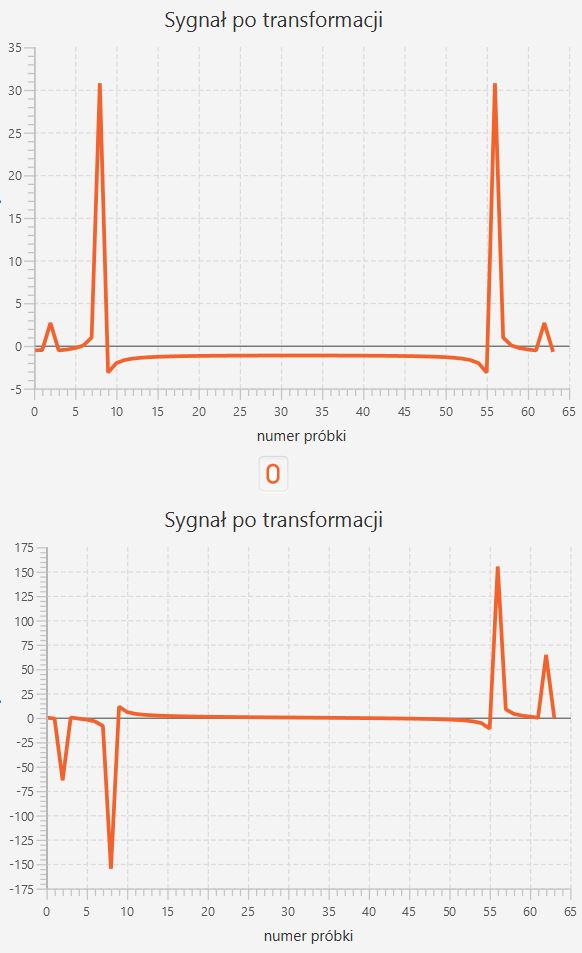
\includegraphics[width=.8\linewidth]{FFT-S1-W1}
	\caption{Wykresy w formie W1 FFT dla sygnału S1. Czas obliczania: 233199}
	\label{S3_sygnal}
\end{figure}
\begin{figure}[H]
	\centering
	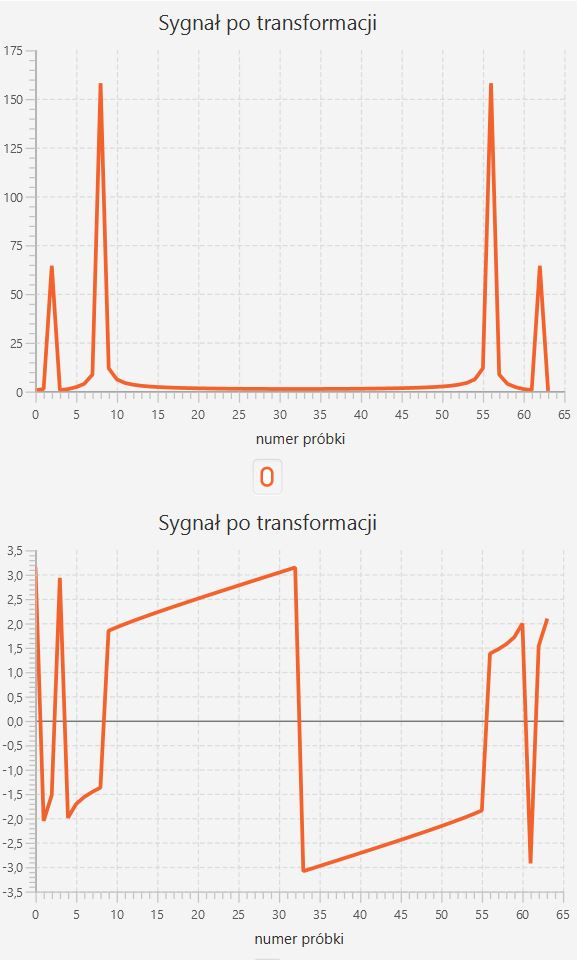
\includegraphics[width=.8\linewidth]{FFT-S1-W2}
	\caption{Wykresy w formie W2 FFT dla sygnału S1. Czas obliczania: 102800}
	\label{S3_sygnal}
\end{figure}


\begin{figure}[H]
	\centering
	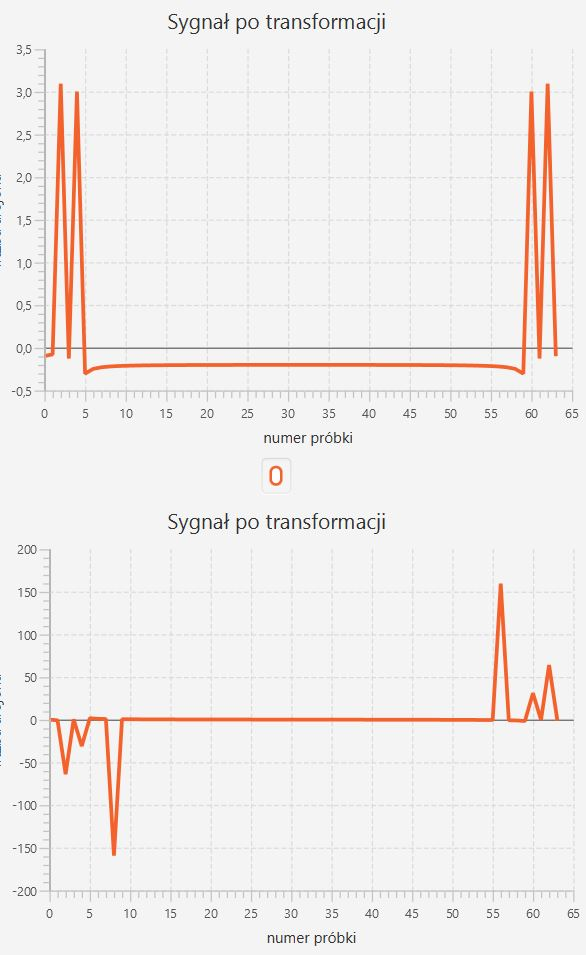
\includegraphics[width=.8\linewidth]{DFT-S2-W1}
	\caption{Wykresy w formie W1 DFT dla sygnału S2. Czas obliczania: 1128499}
	\label{S3_sygnal}
\end{figure}
\begin{figure}[H]
	\centering
	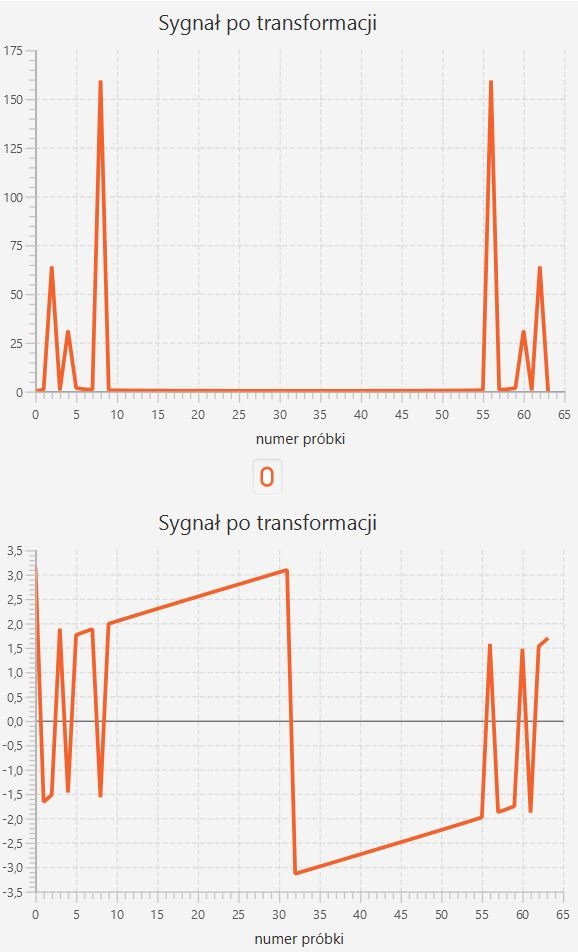
\includegraphics[width=.8\linewidth]{DFT-S2-W2}
	\caption{Wykresy w formie W2 DFT dla sygnału S2. Czas obliczania: 2854500}
	\label{S3_sygnal}
\end{figure}
\begin{figure}[H]
	\centering
	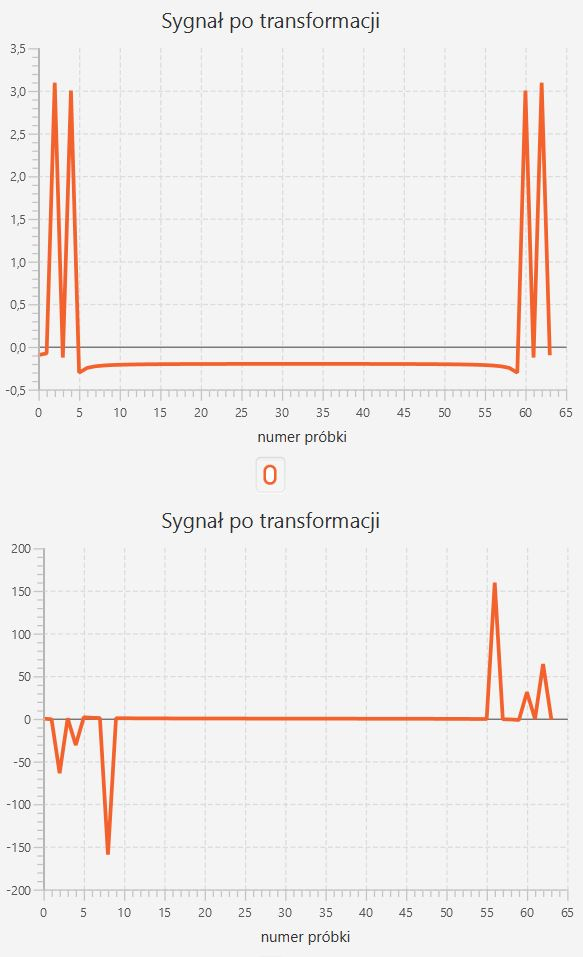
\includegraphics[width=.8\linewidth]{FFT-S2-W1}
	\caption{Wykresy w formie W1 FFT dla sygnału S2. Czas obliczania: 79100}
	\label{S3_sygnal}
\end{figure}
\begin{figure}[H]
	\centering
	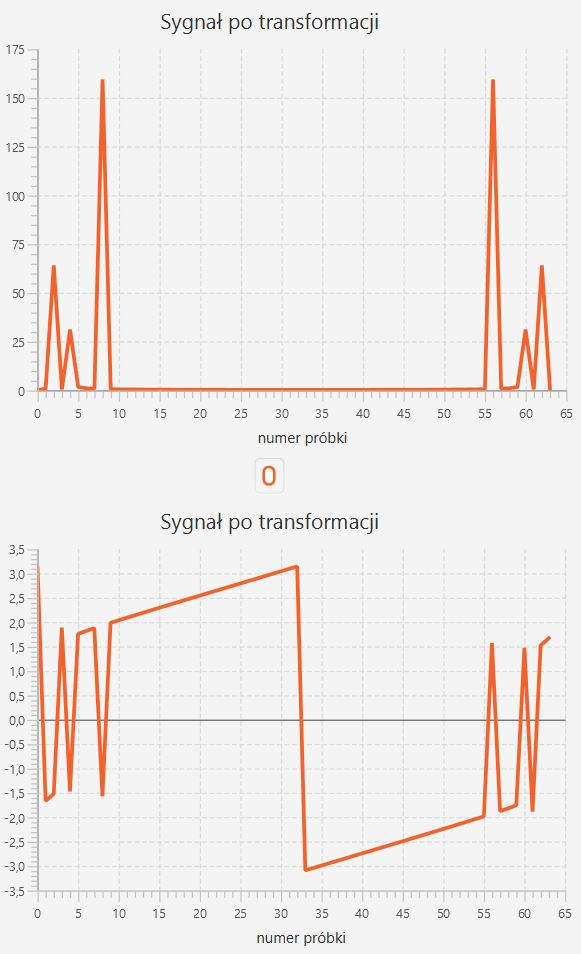
\includegraphics[width=.8\linewidth]{FFT-S2-W2}
	\caption{ Wykresy w formie W2 FFT dla sygnału S2. Czas obliczania: 97300}
	\label{S3_sygnal}
\end{figure}


\begin{figure}[H]
	\centering
	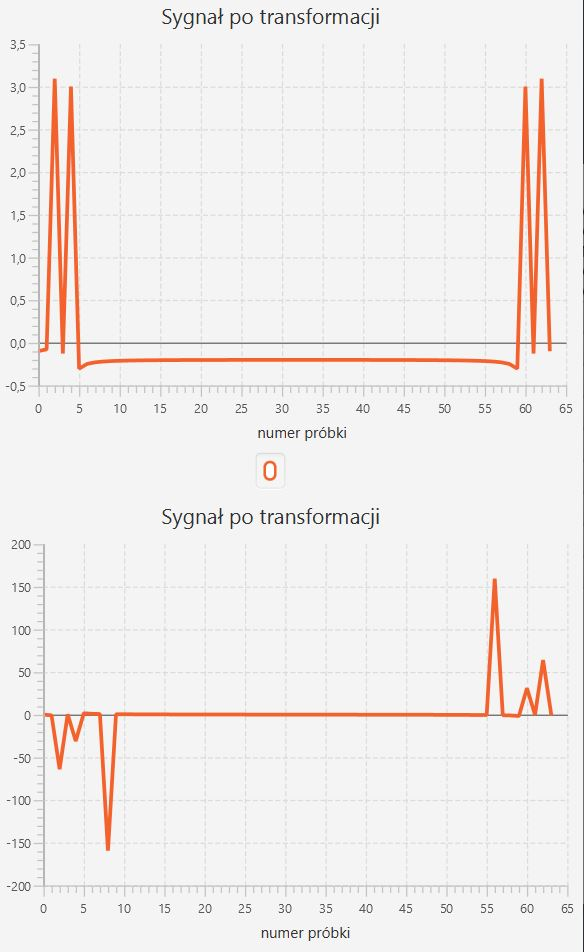
\includegraphics[width=.8\linewidth]{DFT-S3-W1}
	\caption{Wykresy w formie W1 DFT dla sygnału S3. Czas obliczania: 1250000}
	\label{S3_sygnal}
\end{figure}
\begin{figure}[H]
	\centering
	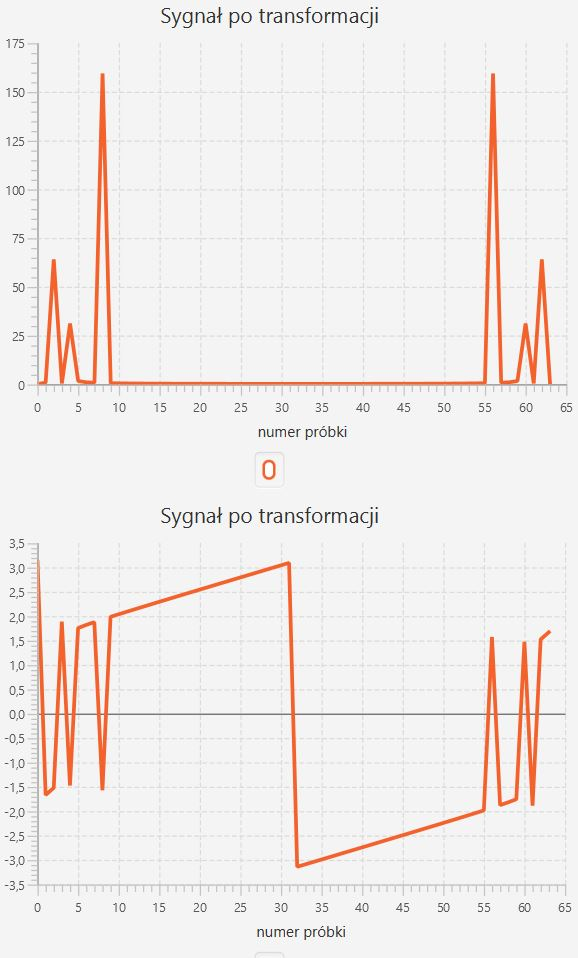
\includegraphics[width=.8\linewidth]{DFT-S3-W2}
	\caption{Wykresy w formie W2 DFT dla sygnału S3. Czas obliczania: 1404800}
	\label{S3_sygnal}
\end{figure}
\begin{figure}[H]
	\centering
	\includegraphics[width=.8\linewidth]{FFT-S3-W1}
	\caption{Wykresy w formie W1 FFT dla sygnału S3. Czas obliczania: 86600}
	\label{S3_sygnal}
\end{figure}
\begin{figure}[H]
	\centering
	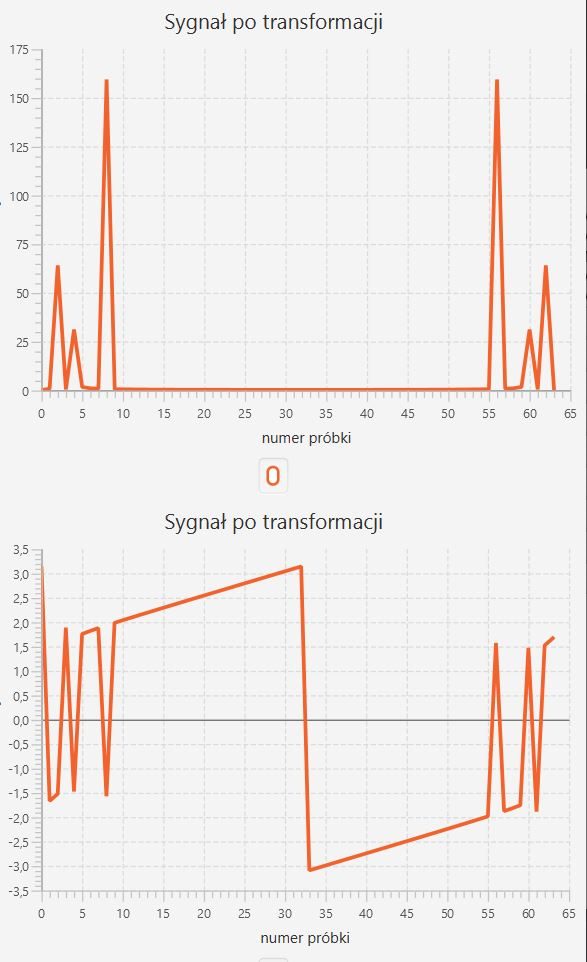
\includegraphics[width=.8\linewidth]{FFT-S3-W2}
	\caption{Wykresy w formie W2 FFT dla sygnału S3. Czas obliczania: 136300}
	\label{S3_sygnal}
\end{figure}


\subsection{Transformacja Falkowa}
W tej sekcji przedstawiony zostanie wykres użyskany z punktów otrzymanych po przeprowadzeniu transformacji falkowej na sygnale S1 dla 64 próbek.
\begin{figure}[H]
	\centering
	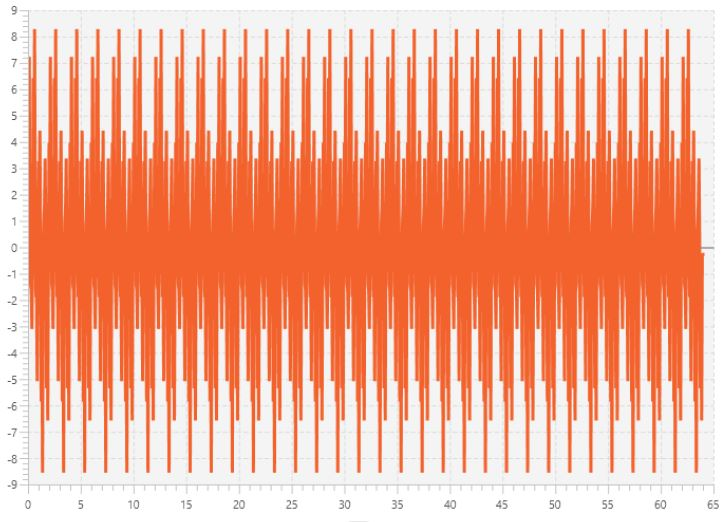
\includegraphics[width=\linewidth]{falkowa-s1}
	\caption{Wykres sygnału S1 po przeprowadzaniu na nim transformacji falkowej}
	\label{s1-falkowa}
\end{figure}
Czas transformacji 0.0001s.

%%%%%%%%%%%%%%%%%%%%%%%%%%%%%%%%%%%%%%%%%%%%%%%%%%%%%%%%%%%%%%%%%%%%%%%%%%%%%%%%%%%%%%%%%%%%%%%%%%%%%%%%%%%%%%%%%

%%%%%%%%%%%%%%%%%%%%%%%%%%%%%%%%%%%%%%%%%%%%%%%%%%%%%%%%%%%%%%%%%%%%%%%%%%%%%%%%%%%%%%%%%%%%%%%%%%%%%%%%%%%%%%%%%
\section{Wnioski}
Wyniki transformacji falkowej wyglądają zupełnie inaczej niż wyniki innych transformat co spowodowane jest tym, iż ta transformata przenosi funkcje w dziedzine czasu. Można również zauważyć, że ta transformacja jest bardzo szybka.
%%%%%%%%%%%%%%%%%%%%%%%%%%%%%%%%%%%%%%%%%%%%%%%%%%%%%%%%%%%%%%%%%%%%%%%%%%%%%%%%%%%%%%%%%%%%%%%%%%%%%%%%%%%%%%%%%
% BIBLIOGRAFIA
%%%%%%%%%%%%%%%%%%%%%%%%%%%%%%%%%%%%%%%%%%%%%%%%%%%%%%%%%%%%%%%%%%%%%%%%%%%%%%%%%%%%%%%%%%%%%%%%%%%%%%%%%%%%%%%%%
\begin{thebibliography}{}
\bibitem{instrukcja} Instrukcja do zadania 4 na stronie przedmiotu. [przeglądany 26.05.2021], Dostępny w: https://ftims.edu.p.lodz.pl/pluginfile.php/14303/mod\_resource/content/0/zadanie4.pdf


\end{thebibliography}



\end{document}
